\documentclass[12pt,letterpaper]{article}

\usepackage[letterpaper,margin=1in]{geometry}
\usepackage{newtxtext,newtxmath}
\usepackage{setspace}
\usepackage{microtype}
\usepackage{lastpage}
\usepackage{fancyhdr}
\usepackage{tikz}
\usepackage{graphicx}
\usepackage{booktabs}
\usepackage{array}
\usepackage{caption}
\usepackage[section]{placeins}
\usepackage[hidelinks]{hyperref}
\usepackage[backend=biber,style=apa,sorting=nyt]{biblatex}
\DeclareLanguageMapping{american}{american-apa}
\addbibresource{references.bib}
\usepackage{enumitem}
\usepackage{titlesec}

\setstretch{1.08}
\setlength{\parindent}{0pt}
\setlength{\parskip}{0.65em}
\setlength{\headheight}{15pt}
\setlist[enumerate]{leftmargin=2em,itemsep=0pt,topsep=0.2em}
\captionsetup{font=it,justification=raggedright,
singlelinecheck=false,skip=4pt}

\titleformat{\section}{\normalfont\bfseries\large}{}{0pt}{\underline}
\titleformat{\subsection}{\normalfont\bfseries\normalsize}{}{0pt}{}
\titlespacing*{\section}{0pt}{1.2em}{0.3em}
\titlespacing*{\subsection}{0pt}{0.8em}{0.2em}

\pagestyle{fancy}
\fancyhf{}
\fancyfoot[R]{\thepage}
\renewcommand{\headrulewidth}{0pt}
\renewcommand{\footrulewidth}{0pt}
\AddToHook{shipout/background}{%
  \begin{tikzpicture}[remember picture,overlay]
    \draw[line width=0.4pt]
      ([xshift=0.5in,yshift=-0.5in]current page.north west)
      rectangle
      ([xshift=-0.5in,yshift=0.5in]current page.south east);
  \end{tikzpicture}}

\newcommand{\wordcount}{1100}

\begin{document}
\begin{center}
\begin{tabular}{>{\raggedright\arraybackslash}p{0.56\textwidth}
>{\centering\arraybackslash}p{0.22\textwidth}}
\toprule
\textbf{Content} & \textbf{Pages} \\
\midrule
Abstract & \pageref{sec:abstract} \\
Introduction & \pageref{sec:introduction} \\
Methodology \& Questions & \pageref{sec:methodology} \\
Results \& Country Evaluation & \pageref{sec:results} \\
Limitations & \pageref{sec:limitations} \\
Conclusion & \pageref{sec:conclusion} \\
Reference list & \pageref{sec:references} \\
Appendix: Use of AI & \pageref{sec:appendix} \\
\bottomrule
\end{tabular}
\end{center}


\section{Abstract}
\label{sec:abstract}
This essay explores whether the world's major coastal economies are meeting their Sustainable Development goals. We will focus on the Goal 14 of Sustainable Development Goals which is Life Below Water. This goal mainly covers issues like pollution, habitats, fisheries, and the effects of climate change on oceans. Big Earth data brings together several abilities - satellite images, vessel tracking, ocean sensors, and models to create comparable information across large regions \parencite{unep2024}. As we know progress around the world is still uneven. In 2024, marine protected areas made up just 8.12 percent of the ocean, and only 62.3 percent of assessed fish stocks were considered biologically sustainable \parencite{un2024}.
 
This essay compares the countries like the United States, China, Japan, Australia, India, and Brazil by looking at indicators for protection, fishing, pollution, and reporting. Some of the countries, such as Australia, the United States, and Brazil have made relatively strong progress in protecting marine areas. China has also improved its coastal monitoring capabilities. Japan and India have strong policy or species programs, but both have gaps in reporting of data. However Coverage alone does not tell the whole story. Factors like Effective management, enforcement, and real ecosystem outcomes are also important.


\section{Introduction}
\label{sec:introduction}
SDG 14 focuses on the conservation and sustainable use of oceans and marine resources. Targets include reducing pollution, protecting ecosystems, ending unsustainable fishing, and strengthening scientific capacity
\parencite{un2015}. As oceans crosses several national boundaries and borders, it is difficult to monitor them on field without the help of technology.

The use of Big Earth data helps to achieve continuous, wide-area observations. Satellites can measure temperature, sea level, pollution, coastal change, and habitat extent. Some systems like Vessel can reveal fishing routes and potentially illegal activity. Buoys, a floating device, can measure water chemistry and biodiversity and then later machine learning models can use these sources to forecasts and trends \parencite{jpl2024}.

This essay evaluates the United States, China, Japan, Australia, India, and Brazil. 
It asks:
\begin{enumerate}
\item What are the indicators to monitor marine pollution, habitats, and fisheries?
\item Which countries show stronger observable progress in achieving SDG 14?
\item What limitations prevents Earth data from proving SDG achievement?
\end{enumerate}

\section{Methodology}
\label{sec:methodology}
This essay uses officially available data from the UN(United Nations), FAO(Food and Agriculture Organization), national agency, and scientific sources. It compares available pollution indicators, fish-stock status, protected-area coverage, and scientific capacity. However, Marine protection is not considered as the sole
indicator of success as only designation does not guarantee effective management or recovery of ecosystems.

We will assess the countries in 3 categories: relatively strong, moderate, or uneven for each indicator. According to my research reporting is uneven, protected-area percentages use different jurisdiction definitions, and fisheries results may refer to national waters or broader regions.

\section{Results and Country Evaluation}
\label{sec:results}
\subsection{Global Monitoring Baseline}
The UN reported that marine protected areas covers merely 8.12 percent of the ocean in May 2024 which is already below the 10-percent 2020 target and the 30-percent 2030 commitment \parencite{un2024}. And we are not moving towards the target. Sustainable fish stocks fell from 90 percent of assessed stocks in 1974 to 62.3 percent in 2021.This is clear sign that we are moving in the wrong direction. Meanwhile, Hazardous effects like ocean heat, coral bleaching, eutrophication, plastic debris, and acidification remain major pressures.

Here, Earth observation is therefore not a single map of ocean health. It produces data for time-series indicators which we can track and analyze. Coastal eutrophication can be estimated from nutrient, chlorophyll, and algae observations using satellite data. Floating debris can be modelled from satellite, drift, and field data. Habitat change can be measured with repeat imagery from satellites, while vessel positions can support IUU-fishing(Illegal, unreported, and unregulated) analysis \parencite{unep2024}.

\begin{figure}[!htb]
\centering
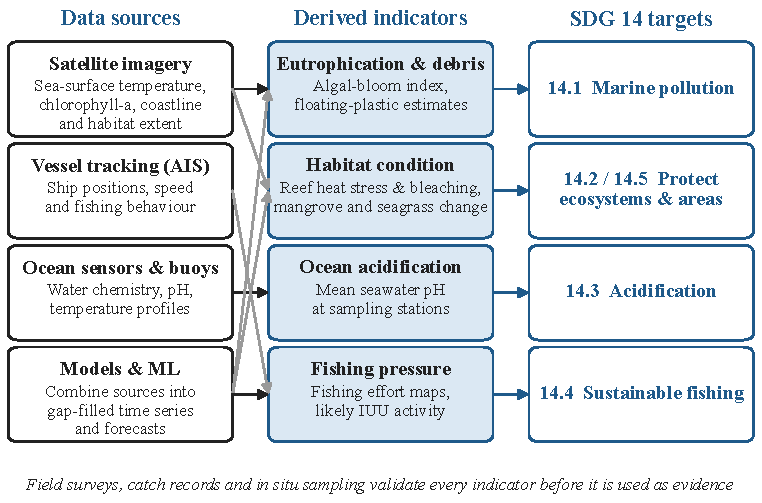
\includegraphics[width=\textwidth]{figures/bigdata_workflow.pdf}
\caption{How Big Earth data sources feed indicators for SDG 14 targets
(created with AI assistance, based on \cite{unep2024} and \cite{jpl2024}).}
\label{fig:workflow}
\end{figure}

\subsection{United States}
NOAA(National Oceanic and Atmospheric Administration) reports nearly 1,000 marine protected areas covering approximately 24 percent of United States waters \parencite{noaa2024}. Recent data shows that in year 2024, 363 stocks were assessed, of which 340 stocks were considered biologically sustainable. This means that 93.7 percent of assessed stocks were sustainable.\parencite{noaa2024fisheries}.

The United States shows relatively strong legal protection and monitoring with regular stock assessment. Areas differ in restriction, however, and designation does not always mean strict no-take protection. Achievement
is strong in monitoring and many fisheries, but it is not fully verified across all states of USA.

\subsection{China}
China reports in total 352 marine protected areas covering almost 9.33 million hectares. In 2024, 83.7 percent of monitored nearshore waters were good or excellent, and no monitored ecosystem category was unhealthy \parencite{china2024,china2025}.

These results indicate improving pollution monitoring and habitat management. However, intensive fisheries and coastal development remain risks that means nearshore results do not measure the whole EEZ or all fish stocks. China is moderate-to-strong, with progress and major remaining pressure.

\subsection{Australia}
Australia had 319 marine protected areas and 11 Indigenous protected areas covering 48.9 percent of its waters in 2024, which will rise to 52 percent after an expansion in coming years \parencite{dcceew2024,dcceew2025}. It uses national fish-stock reports for SDG 14.4.1.

This represents strong protection and visible monitoring. The Great Barrier Reef continues to experience heat stress and bleaching, however. Protection is relatively strong, but climate recovery remains incomplete. Moreover, Australia has a large EEZ and many migratory stocks that are not fully assessed.

\subsection{Brazil}
Brazil reported 26.49 percent of its marine biome protected in 2023, exceeding the 10-percent target \parencite{ipea2024}. It has a large artisanal-fishing sector and extensive offshore protection.

Brazil is strong in designation but uneven in implementation. Enforcement, ecosystem monitoring, and national fish-stock and pollution data require further development.

\subsection{Japan and India}
Japan has advanced marine science, fisheries management and a 30by30 marine protection commitment. Nevertheless, available national reporting does not provide a consistently comparable public marine-protection percentage, and fisheries remain affected by stock and regional pressures.
Japan's achievement is therefore moderate to strong in policy and science, but not fully verified across all SDG indicators.

India had notified 130 marine protected areas and identified 106 coastal and marine biodiversity areas by 2024 \parencite{india2024}. These networks support species and habitat conservation. However, coastal plastic
pollution, eutrophication, high fishing pressure, and inconsistent monitoring indicate only moderate achievement.  Here India is moderate, with strong species and habitat programs but it needs better monitoring and reporting and also must use Earth observation to track progress.

\begin{figure}[!htb]
\centering
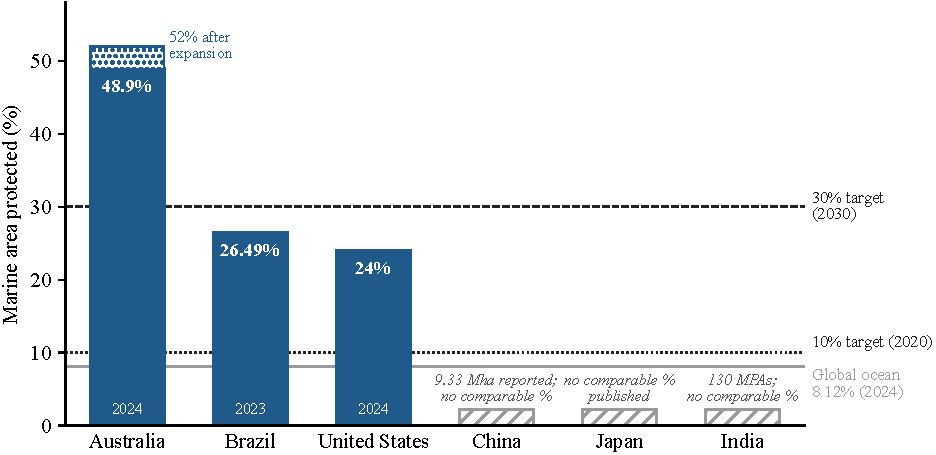
\includegraphics[width=\textwidth]{figures/mpa_coverage.pdf}
\caption{Reported marine protected-area coverage of national waters compared
with the 2020 and 2030 targets. Hatched bars mark countries without a
comparable published percentage. National figures as cited in the country
sections; global coverage from \cite{un2024}.}
\label{fig:mpa}
\end{figure}

\begin{table}[htbp]
\centering
\caption{Comparative assessment of major coastal economies.}
\label{tab:countries}
\begin{tabular}{p{0.12\textwidth}p{0.23\textwidth}p{0.23\textwidth}p{0.25\textwidth}}
\toprule
Country & Strong evidence & Main weakness & Overall result \\
\midrule
United States & MPA coverage and stock assessment & MPA effectiveness varies &
Strong monitoring; uneven national implementation \\
China & Nearshore water quality and protected habitats & Scale and pollution remain &
Improving, moderate-to-strong \\
Australia & 52\% marine-area coverage & Climate damage and reef bleaching &
Strong protection, incomplete ecosystem recovery \\
Brazil & 26.49\% marine-biome coverage & Enforcement and fish-stock data &
Strong designation, uneven implementation \\
Japan & Scientific capacity and policy & Comparable public progress is limited &
Moderate-to-strong \\
India & 130 MPAs and species programmes & Pollution and fisheries reporting &
Moderate, with large improvement needed \\
\bottomrule
\end{tabular}
\end{table}

\section{Limitations}
\label{sec:limitations}
As we have seen, protected-area coverage is an imperfect indicator because some areas permit extractive activities or are poorly managed. Fisheries status may cover only assessed stocks, while national totals omit shared or highly migratory stocks which are not fully accounted for. Pollution measurements may also differ in resolution and methodology.

Earth data can show spatial change in marine environments, but cannot establish cause alone. Causality requires field surveys, catch records, and in situ monitoring. Satellite observations need field validation, while illegal fishing analyses can produce false accusations if vessel data are incomplete and inaccurate. Countries should publish uncertainty of their used methods, data coverage, and enforcement methods rather than treat remote-sensing results as definitive.

Finally, no six-country comparison covers all major actors. Even quite small nations with small economies or island territories may contribute disproportionately to biodiversity and receive insufficient monitoring resources.

\section{Conclusion}
\label{sec:conclusion}
Major countries have achieved SDG 14 unevenly. However overall effect shows countries are making effort but most of them lacks effective management. Australia has the strongest visible protected-area coverage, the United States has strong fisheries assessment and a large MPA network, and Brazil has exceeded the 10-percent marine-protection target. China shows improving national pollution monitoring, while Japan and India combine stronger policy and species programmes with reporting or implementation gaps.

Big Earth data make these differences measurable and actionable. Satellite and sensor records reveal pollution, habitat change, bleaching, and climate stress, while vessel data support fisheries enforcement. Combined with in-field surveys, catch records, and public dashboards, these data can evaluate whether protected areas and regulations produce outcomes. Marine ecosystem's health can also be tracked over time, and countries can be held accountable for their SDG 14 commitments. And effect of country's effort can be measured by the recovery of marine ecosystem and not only by the percentage of ocean formally protected.

The evidence shows that designation alone is insufficient. Countries need effective management, transparent enforcement, open data, scientific funding, and cooperation in international waters where they can work together. In addition, countries must monitor fish stocks and pollution consistently. And they should publish their data and progress regularly. These measures would allow SDG 14 achievement to be judged by ecological recovery and not only by the percentage of ocean formally protected.

\clearpage
\section*{References}
\label{sec:references}
\addcontentsline{toc}{section}{Reference list}
\printbibliography[heading=none]

\clearpage
\section*{Appendix: Use of AI}
\label{sec:appendix}
Figures~\ref{fig:workflow} and~\ref{fig:mpa} in this essay were generated using AI coding assistance. The AI tool
(Claude Code, Anthropic) wrote the Python code (matplotlib) that draws both
figures. All values shown in the coverage chart come from the sources cited in
this essay, and the author reviewed both figures for accuracy.
\end{document}
